\section{strlen()}
\myindex{\CStandardLibrary!strlen()}

\ifdefined\ENGLISH
Let's talk about loops one more time. Often, the \TT{strlen()} 
function
\footnote{counting the characters in a string in the C language} 
is implemented using a \TT{while()} statement.
Here is how it is done in the MSVC standard libraries:
\fi

\ifdefined\RUSSIAN
Ещё немного о циклах. Часто функция \TT{strlen()}
\footnote{подсчет длины строки в Си}
реализуется при помощи \TT{while()}.
Например, вот как это сделано в стандартных библиотеках MSVC:
\fi

\lstinputlisting{patterns/10_strings/1_strlen/ex1.c}

% subsections
\EN{\subsubsection{x86}

\myparagraph{\NonOptimizing MSVC}

Let's compile:

\lstinputlisting{patterns/10_strings/1_strlen/10_1_msvc_EN.asm}

\myindex{x86!\Instructions!MOVSX}
\myindex{x86!\Instructions!TEST}

We get two new instructions here: \MOVSX and \TEST.

\label{MOVSX}

The first one---\MOVSX---takes a byte from an address in memory and stores the value in a 32-bit register. 
\MOVSX stands for \IT{MOV with Sign-Extend}. 
\MOVSX sets the rest of the bits, from the 8th to the 31th, 
to 1 if the source byte is \IT{negative} or to 0 if is \IT{positive}.

And here is why.

By default, the \Tchar type is signed in MSVC and GCC. If we have two values of which one is \Tchar 
and the other is \Tint, (\Tint is signed too), and if the first value contain -2 (coded as \TT{0xFE}) 
and we just copy this byte into the \Tint container, it makes \TT{0x000000FE}, and this 
from the point of signed \Tint view is 254, but not -2. In signed int, -2 is coded as \TT{0xFFFFFFFE}. 
So if we need to transfer \TT{0xFE} from a variable of \Tchar type to \Tint, 
we need to identify its sign and extend it. That is what \MOVSX does.

You can also read about it in \q{\IT{\SignedNumbersSectionName}} section~(\myref{sec:signednumbers}).

It's hard to say if the compiler needs to store a \Tchar variable in \EDX, it could just take a 8-bit register part 
(for example \DL). Apparently, the compiler's \gls{register allocator} works like that.

\myindex{ARM!\Instructions!TEST}

Then we see \TT{TEST EDX, EDX}. 
You can read more about the \TEST instruction in the section about bit fields~(\myref{sec:bitfields}).
Here this instruction just checks if the value in \EDX equals to 0.

\myparagraph{\NonOptimizing GCC}

Let's try GCC 4.4.1:

\lstinputlisting{patterns/10_strings/1_strlen/10_3_gcc.asm}

\label{movzx}
\myindex{x86!\Instructions!MOVZX}

The result is almost the same as in MSVC, but here we see \MOVZX instead of \MOVSX. 
\MOVZX stands for \IT{MOV with Zero-Extend}. 
This instruction copies a 8-bit or 16-bit value into a 32-bit register and sets the rest of the bits to 0. 
In fact, this instruction is convenient only because it enable us to replace this instruction pair:\\
\TT{xor eax, eax / mov al, [...]}.

On the other hand, it is obvious that the compiler could produce this code: \\
\TT{mov al, byte ptr [eax] / test al, al}---it is almost the same, however, 
the highest bits of the \EAX register will contain random noise. 
But let's think it is compiler's drawback---it cannot produce more understandable code. 
Strictly speaking, the compiler is not obliged to emit understandable (to humans) code at all.

\myindex{x86!\Instructions!SETcc}

The next new instruction for us is \SETNZ. 
Here, if \AL doesn't contain zero, \TT{test al, al} 
sets the \ZF flag to 0, but \SETNZ, if \TT{ZF==0} (\IT{NZ} stands for \IT{not zero}) sets \AL to 1.
Speaking in natural language, \IT{if \AL is not zero, let's jump to loc\_80483F0}. 
The compiler emits some redundant code, but let's not forget that the optimizations are turned off.

\myparagraph{\Optimizing MSVC}
\label{strlen_MSVC_Ox}

Now let's compile all this in MSVC 2012, with optimizations turned on (\Ox):

\lstinputlisting[caption=\Optimizing MSVC 2012 /Ob0]{patterns/10_strings/1_strlen/10_2_EN.asm}

Now it is all simpler.
Needless to say, the compiler could use registers with such efficiency
only in small functions with a few local variables.

\myindex{x86!\Instructions!INC}
\myindex{x86!\Instructions!DEC}
\INC/\DEC---are \gls{increment}/\gls{decrement} instructions, in other words: add or substract 1 to/from a variable.

\clearpage
\subsubsectionold{\Optimizing MSVC + \olly}
\myindex{\olly}

We can try this (optimized) example in \olly.  Here is the first iteration:

\begin{figure}[H]
\centering
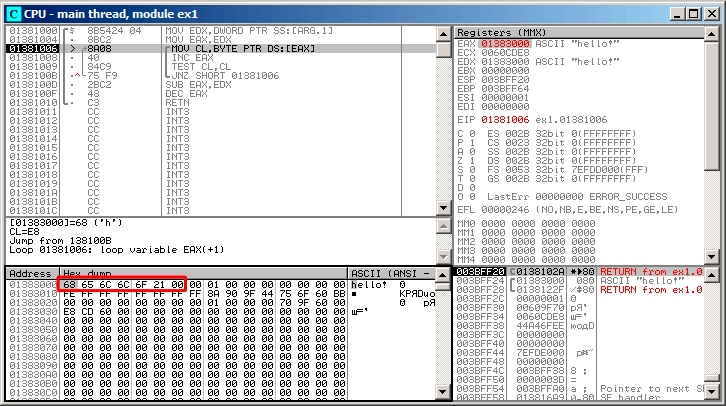
\includegraphics[scale=\FigScale]{patterns/10_strings/1_strlen/olly1.png}
\caption{\olly: first iteration start}
\label{fig:strlen_olly_1}
\end{figure}

We see that \olly found a loop and, for convenience, \IT{wrapped} its instructions in brackets.
By clicking the right button on \EAX, we can choose 
\q{Follow in Dump} and the memory window scrolls to the right place.
Here we can see the string \q{hello!} in memory.
There is at least
one zero byte after it and then random garbage.

If \olly sees a register with a valid address in it, that points to some string, 
it is shown as a string.

\clearpage
Let's press F8 (\stepover) a few times, to get to the start of the body of the loop:

\begin{figure}[H]
\centering
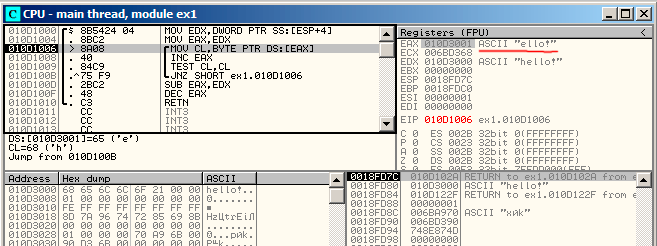
\includegraphics[scale=\FigScale]{patterns/10_strings/1_strlen/olly2.png}
\caption{\olly: second iteration start}
\label{fig:strlen_olly_2}
\end{figure}

We see that \EAX contains the address of the second character in the string.

\clearpage

We have to press F8 enough number of times in order to escape from the loop:

\begin{figure}[H]
\centering
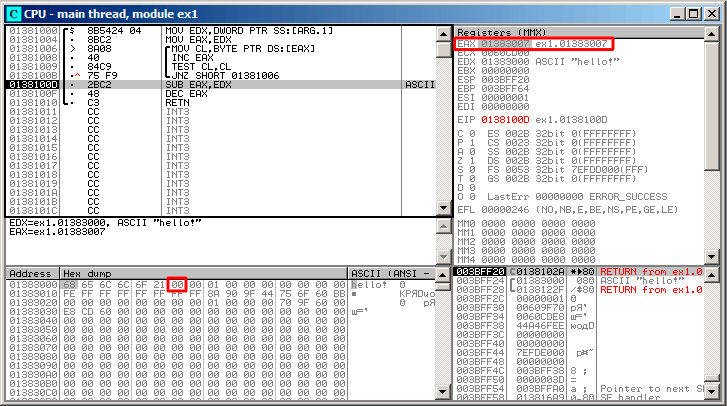
\includegraphics[scale=\FigScale]{patterns/10_strings/1_strlen/olly3.png}
\caption{\olly: pointers difference to be calculated now}
\label{fig:strlen_olly_3}
\end{figure}

We see that \EAX now contains the address of zero byte that's right after the string.
Meanwhile, \EDX hasn't changed,
so it still pointing to the start of the string.

The difference between these two addresses is being calculated now.

\clearpage
The \SUB instruction just got executed:

\begin{figure}[H]
\centering
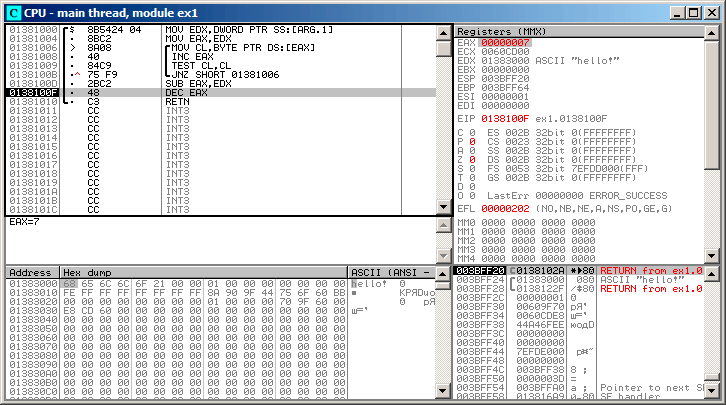
\includegraphics[scale=\FigScale]{patterns/10_strings/1_strlen/olly4.png}
\caption{\olly: \EAX to be decremented now}
\label{fig:strlen_olly_4}
\end{figure}

The difference of pointers is in the \EAX register now---7.
Indeed, the length of the \q{hello!} string is 6, 
but with the zero byte included\EMDASH{}7.
But \TT{strlen()} must return the number of non-zero characters in the string.
So the decrement executes and then the function returns.


\myparagraph{\Optimizing GCC}

Let's check GCC 4.4.1 with optimizations turned on (\Othree key):

\lstinputlisting{patterns/10_strings/1_strlen/10_3_gcc_O3.asm}
 
Here GCC is almost the same as MSVC, except for the presence of \MOVZX.
However, here \MOVZX could be replaced with\\
\TT{mov dl, byte ptr [eax]}.

Perhaps it is simpler for GCC's code generator to \IT{remember} 
the whole 32-bit \EDX register 
is allocated for a \Tchar variable and it then can be sure that the highest bits has no any noise 
at any point.

\label{strlen_NOT_ADD}
\myindex{x86!\Instructions!NOT}
\myindex{x86!\Instructions!XOR}

After that we also see a new instruction---\NOT. This instruction inverts all bits in the operand. \\
You can say that it is a synonym to the \TT{XOR ECX, 0ffffffffh} instruction. 
\NOT and the following \ADD calculate the pointer difference and subtract 1, just in a different way. 
At the start \ECX, where the pointer to \IT{str} is stored, gets inverted and 1 is subtracted from it.

See also: \q{\SignedNumbersSectionName}~(\myref{sec:signednumbers}).
 
In other words, at the end of the function just after loop body, these operations are executed:

\begin{lstlisting}
ecx=str;
eax=eos;
ecx=(-ecx)-1; 
eax=eax+ecx
return eax
\end{lstlisting}

\dots~and this is effectively equivalent to:

\begin{lstlisting}
ecx=str;
eax=eos;
eax=eax-ecx;
eax=eax-1;
return eax
\end{lstlisting}

Why did GCC decide it would be better? Hard to guess. 
But perhaps the both variants are equivalent in efficiency.
}
\RU{\subsection{x86}

\subsubsection{\NonOptimizing MSVC}

Итак, компилируем:

\lstinputlisting{patterns/10_strings/1_strlen/10_1_msvc_RU.asm}

\myindex{x86!\Instructions!MOVSX}
\myindex{x86!\Instructions!TEST}
Здесь две новых инструкции: \MOVSX и \TEST.

\label{MOVSX}
О первой. \MOVSX предназначена для того, чтобы взять байт из какого-либо места в памяти и положить его, 
в нашем случае, в регистр \EDX. 
Но регистр \EDX~--- 32-битный. \MOVSX означает \IT{MOV with Sign-Extend}. 
Оставшиеся биты с 8-го по 31-й \MOVSX сделает единицей, если исходный байт в памяти имеет знак \IT{минус}, 
или заполнит нулями, если знак \IT{плюс}.

И вот зачем всё это.

По умолчанию в MSVC и GCC тип \Tchar~--- знаковый. Если у нас есть две переменные, одна \Tchar, а другая \Tint 
(\Tint тоже знаковый), и если в первой переменной лежит -2 (что кодируется как \TT{0xFE}) и мы просто 
переложим это в \Tint, 
то там будет \TT{0x000000FE}, а это, с точки зрения \Tint, даже знакового, будет 254, но никак не -2. 
-2 в переменной \Tint кодируется как \TT{0xFFFFFFFE}. Для того чтобы значение \TT{0xFE} из переменной типа 
\Tchar переложить 
в знаковый \Tint с сохранением всего, нужно узнать его знак и затем заполнить остальные биты. 
Это делает \MOVSX.

См. также об этом раздел
 \q{\IT{\SignedNumbersSectionName}}~(\myref{sec:signednumbers}).

Хотя конкретно здесь компилятору вряд ли была особая надобность хранить значение \Tchar в регистре \EDX, 
а не его восьмибитной части, скажем \DL. Но получилось, как получилось. Должно быть 
\gls{register allocator} компилятора сработал именно так.

\myindex{ARM!\Instructions!TEST}
Позже выполняется \TT{TEST EDX, EDX}. 
Об инструкции \TEST читайте в разделе о битовых полях~(\myref{sec:bitfields}).
Конкретно здесь эта инструкция просто проверяет состояние регистра \EDX на 0.

\ifdefined\IncludeGCC
\subsubsection{\NonOptimizing GCC}

Попробуем GCC 4.4.1:

\lstinputlisting{patterns/10_strings/1_strlen/10_3_gcc.asm}

\label{movzx}
\myindex{x86!\Instructions!MOVZX}
Результат очень похож на MSVC, только здесь используется \MOVZX, а не \MOVSX. 
\MOVZX означает \IT{MOV with Zero-Extend}. Эта инструкция перекладывает какое-либо значение 
в регистр и остальные биты выставляет в 0.
Фактически, преимущество этой инструкции только в том, что она позволяет 
заменить две инструкции сразу: \TT{xor eax, eax / mov al, [...]}.

С другой стороны, нам очевидно, что здесь можно было бы написать вот так: 
\TT{mov al, byte ptr [eax] / test al, al}~--- это тоже самое, хотя старшие биты \EAX будут \q{замусорены}. 
Но будем считать, что это погрешность компилятора~--- 
он не смог сделать код более экономным или более понятным. 
Строго говоря, компилятор вообще не нацелен на то, чтобы генерировать понятный (для человека) код.

\myindex{x86!\Instructions!SETcc}
Следующая новая инструкция для нас~--- \SETNZ. В данном случае, если в \AL был не ноль, 
то \TT{test al, al} выставит флаг \ZF в 0, а \SETNZ, если \TT{ZF==0} 
(\IT{NZ} значит \IT{not zero}) выставит 1 в \AL. 
Смысл этой процедуры в том, что 
\IT{если AL не ноль, выполнить переход на} \TT{loc\_80483F0}.
Компилятор выдал немного избыточный код, но не будем забывать, что оптимизация выключена.

\fi

\subsubsection{\Optimizing MSVC}
\label{strlen_MSVC_Ox}

Теперь скомпилируем всё то же самое в MSVC 2012, но с включенной оптимизацией (\Ox)
:

\lstinputlisting[caption=\Optimizing MSVC 2012 /Ob0]{patterns/10_strings/1_strlen/10_2_RU.asm}

Здесь всё попроще стало. Но следует отметить, что компилятор обычно может так хорошо использовать регистры 
только на небольших функциях с небольшим количеством локальных переменных.

\myindex{x86!\Instructions!INC}
\myindex{x86!\Instructions!DEC}
\INC/\DEC --- это инструкции \glslink{increment}{инкремента}-\glslink{decrement}{декремента}. Попросту говоря~--- 
увеличить на единицу или уменьшить.

\ifdefined\IncludeOlly
\clearpage
\subsubsectionold{\Optimizing MSVC + \olly}
\myindex{\olly}

Можем попробовать этот (соптимизированный) пример в \olly.  Вот самая первая итерация:

\begin{figure}[H]
\centering
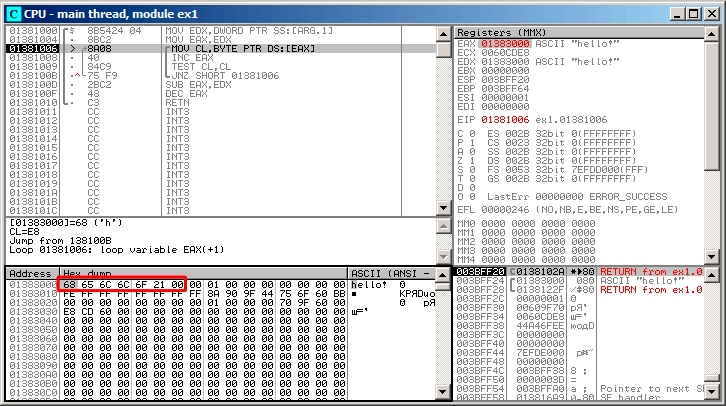
\includegraphics[scale=\FigScale]{patterns/10_strings/1_strlen/olly1.png}
\caption{\olly: начало первой итерации}
\label{fig:strlen_olly_1}
\end{figure}

Видно, что \olly обнаружил цикл и, для удобства, \IT{свернул} инструкции тела цикла в скобке.

Нажав правой кнопкой на \EAX, можно выбрать \q{Follow in Dump} 
и позиция в окне памяти будет как раз там, где надо.

Здесь мы видим в памяти строку \q{hello!}.
После неё имеется как минимум 1 нулевой байт, затем случайный мусор.
Если \olly видит, что в регистре содержится адрес какой-то строки, он показывает эту строку.

\clearpage
Нажмем F8 (\stepover) столько раз, чтобы текущий адрес снова был в начале тела цикла:

\begin{figure}[H]
\centering
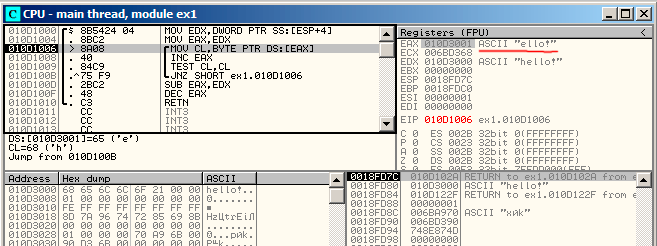
\includegraphics[scale=\FigScale]{patterns/10_strings/1_strlen/olly2.png}
\caption{\olly: начало второй итерации}
\label{fig:strlen_olly_2}
\end{figure}

Видно, что \EAX уже содержит адрес второго символа в строке.

\clearpage
Будем нажимать F8 достаточное количество раз, чтобы выйти из цикла:

\begin{figure}[H]
\centering
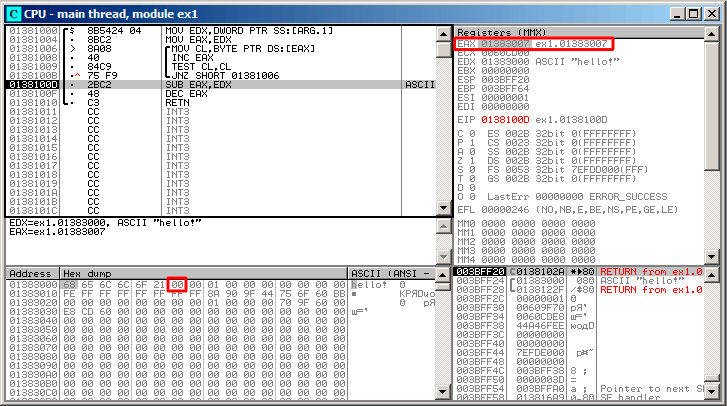
\includegraphics[scale=\FigScale]{patterns/10_strings/1_strlen/olly3.png}
\caption{\olly: сейчас будет вычисление разницы указателей}
\label{fig:strlen_olly_3}
\end{figure}

Увидим, что \EAX теперь содержит адрес нулевого байта, следующего сразу за строкой.

А \EDX так и не менялся~--- он всё ещё указывает на начало строки.
Здесь сейчас будет вычисляться разница между этими двумя адресами.

\clearpage
Инструкция \SUB исполнилась:

\begin{figure}[H]
\centering
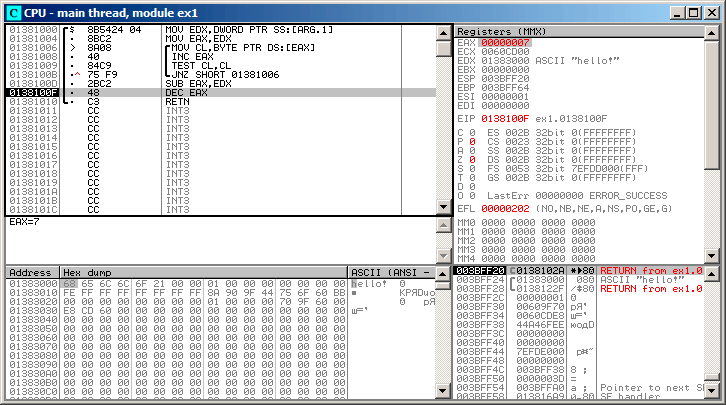
\includegraphics[scale=\FigScale]{patterns/10_strings/1_strlen/olly4.png}
\caption{\olly: сейчас будет декремент \EAX}
\label{fig:strlen_olly_4}
\end{figure}

Разница указателей сейчас в регистре \EAX~--- 7.

Действительно, длина строки \q{hello!}~--- 6, 
но вместе с нулевым байтом\EMDASH{}7.
Но \TT{strlen()} должна возвращать количество ненулевых символов в строке.
Так что сейчас будет исполняться декремент и выход из функции.


\fi

\ifdefined\IncludeGCC
\subsubsection{\Optimizing GCC}

Попробуем GCC 4.4.1 с включенной оптимизацией (ключ \Othree):

\lstinputlisting{patterns/10_strings/1_strlen/10_3_gcc_O3.asm}

Здесь GCC не очень отстает от MSVC за исключением наличия \MOVZX. 

Впрочем, \MOVZX здесь явно можно заменить на \TT{mov dl, byte ptr [eax]}.

Но возможно, компилятору GCC просто проще помнить, что у него под переменную типа \Tchar отведен целый 
32-битный регистр \EDX и быть уверенным в том, что старшие биты регистра не будут замусорены.

\label{strlen_NOT_ADD}
\myindex{x86!\Instructions!NOT}
\myindex{x86!\Instructions!XOR}
Далее мы видим новую для нас инструкцию \NOT. Эта инструкция инвертирует все биты в операнде. 
Можно сказать, что здесь это синонимично инструкции \TT{XOR ECX, 0ffffffffh}. 
\NOT и следующая за ней инструкция \ADD вычисляют разницу указателей и отнимают от результата единицу. 
Только происходит это слегка по-другому. Сначала \ECX, где хранится указатель на \IT{str}, 
инвертируется и от него отнимается единица.
См. также раздел: \q{\SignedNumbersSectionName}~(\myref{sec:signednumbers}).

Иными словами, в конце функции, после цикла, происходит примерно следующее: 

\begin{lstlisting}
ecx=str;
eax=eos;
ecx=(-ecx)-1; 
eax=eax+ecx
return eax
\end{lstlisting}

\dots~что эквивалентно:

\begin{lstlisting}
ecx=str;
eax=eos;
eax=eax-ecx;
eax=eax-1;
return eax
\end{lstlisting}

Но почему GCC решил, что так будет лучше? Трудно угадать.
Но наверное, оба эти варианта работают примерно одинаково в плане эффективности и скорости.

\fi
}
\ifdefined\IncludeARM
\subsection{ARM}

% subsubsections
\EN{\subsubsectionold{32-bit ARM}

\myparagraphold{\NonOptimizingXcodeIV (\ARMMode)}

\lstinputlisting[caption=\NonOptimizingXcodeIV (\ARMMode),label=ARM_leaf_example7]{patterns/10_strings/1_strlen/ARM/xcode_ARM_O0_EN.asm}

Non-optimizing LLVM generates too much code, however, here we can see how the function works with 
local variables in the stack.
There are only two local variables in our function: \IT{eos} and \IT{str}.
In this listing, generated by \IDA, we have manually renamed \IT{var\_8} and \IT{var\_4} to \IT{eos} and \IT{str}.

The first instructions just saves the input values into both \IT{str} and \IT{eos}.

The body of the loop starts at label \IT{loc\_2CB8}.

The first three instruction in the loop body (\TT{LDR}, \ADD, \TT{STR}) load the value of \IT{eos} into \Reg{0}. 
Then the value is \glslink{increment}{incremented} and saved back into \IT{eos}, which is located in the stack.

\myindex{ARM!\Instructions!LDRSB}
The next instruction,  \TT{LDRSB R0, [R0]} (\q{Load Register Signed Byte}), loads a byte from memory at the address stored in \Reg{0} and sign-extends it to 32-bit
\footnote{The Keil compiler treats the \Tchar type as signed, just like MSVC and GCC.}.
\myindex{x86!\Instructions!MOVSX}
This is similar to the \MOVSX instruction in x86.

The compiler treats this byte as signed since the \Tchar type is signed according to the C standard.
It was already written about it~(\myref{MOVSX}) in this section, in relation to x86.

\myindex{Intel!8086}
\myindex{Intel!8080}
\myindex{ARM}

It has to be noted that it is impossible to use 8- or 16-bit part 
of a 32-bit register in ARM separately of the whole register,
as it is in x86.

Apparently, it is because x86 has a huge history of backwards compatibility with its ancestors 
up to the 16-bit 8086 and even 8-bit 8080,
but ARM was developed from scratch as a 32-bit RISC-processor.

Consequently, in order to process separate bytes in ARM, one has to use 32-bit registers anyway.

So, \TT{LDRSB} loads bytes from the string into \Reg{0}, one by one.
The following \CMP and \ac{BEQ} instructions check if the loaded byte is 0.
If it's not 0, control passes to the start of the body of the loop.
And if it's 0, the loop ends.

At the end of the function, the difference between 
\IT{eos} and \IT{str} is calculated, 1 is subtracted from it, and resulting value is returned
via \Reg{0}.

N.B. Registers were not saved in this function.
\myindex{ARM!\Registers!scratch registers}

That's because in the ARM calling convention registers \Reg{0}-\Reg{3} are \q{scratch registers}, 
intended for arguments passing,
and we're not required to restore their value when the function exits, 
since the calling function will not use them anymore.
Consequently, they may be used for anything we want.

No other registers are used here, so that is why we have nothing to save on the stack.

Thus, control may be returned back to calling function by a simple jump (\TT{BX}),
to the address in the \ac{LR} register.

\myparagraphold{\OptimizingXcodeIV (\ThumbMode)}

\lstinputlisting[caption=\OptimizingXcodeIV (\ThumbMode)]{patterns/10_strings/1_strlen/ARM/xcode_thumb_O3.asm}

As optimizing LLVM concludes, \IT{eos} and \IT{str} do not need space on the stack, and can always be stored in registers.

Before the start of the loop body, \IT{str} is always in \Reg{0}, 
and \IT{eos}---in \Reg{1}.

\myindex{ARM!\Instructions!LDRB.W}
The \TT{LDRB.W R2, [R1],\#1} instruction loads a byte from the memory at the address stored in \Reg{1}, to \Reg{2}, sign-extending it to a 32-bit value, but not just that.
\TT{\#1} at the instruction's end is implies \q{Post-indexed addressing}, which means that 1 is to be added to \Reg{1} after the byte is loaded.
Read more about it: \myref{ARM_postindex_vs_preindex}.

Then you can see \CMP and \ac{BNE} in the body of the loop, these instructions continue looping until 0 is found in the string.

\myindex{ARM!\Instructions!MVNS}
\myindex{x86!\Instructions!NOT}
\TT{MVNS}\footnote{MoVe Not} (inverts all bits, like \NOT in x86) and \ADD instructions compute $eos - str - 1$.
In fact, these two instructions compute $R0 = ~str + eos$, 
which is effectively equivalent to what was in the source code, and why it is so, was already explained here
~(\myref{strlen_NOT_ADD}).

Apparently, LLVM, just like GCC, concludes that this code can be shorter (or faster).

\myparagraphold{\OptimizingKeilVI (\ARMMode)}

\lstinputlisting[caption=\OptimizingKeilVI (\ARMMode),label=ARM_leaf_example6]{patterns/10_strings/1_strlen/ARM/Keil_ARM_O3.asm}

\myindex{ARM!\Instructions!SUBEQ}

Almost the same as what we saw before, with the exception that the $str - eos - 1$ 
expression can be computed not at the function's end, but right in the body of the loop.
The \TT{-EQ} suffix, as we may recall, implies that the instruction executes only if the operands in
the \CMP that was executed before were equal to each other.
Thus, if \Reg{0} contains 0, both \TT{SUBEQ} instructions executes and result is left in the \Reg{0} register.

}
\RU{\subsubsection{32-битный ARM}

\myparagraph{\NonOptimizingXcodeIV (\ARMMode)}

\lstinputlisting[caption=\NonOptimizingXcodeIV (\ARMMode),label=ARM_leaf_example7]{patterns/10_strings/1_strlen/ARM/xcode_ARM_O0_RU.asm}

Неоптимизирующий LLVM генерирует слишком много кода. Зато на этом примере можно посмотреть, 
как функции работают с локальными переменными в стеке.

В нашей функции только локальных переменных две\EMDASH{}это два указателя:
\IT{eos} и \IT{str}.
В этом листинге сгенерированном при помощи \IDA мы переименовали \IT{var\_8} и \IT{var\_4} в \IT{eos} и \IT{str} вручную.%

Итак, первые несколько инструкций просто сохраняют входное значение в обоих переменных \IT{str} и \IT{eos}.

С метки \IT{loc\_2CB8} начинается тело цикла.

Первые три инструкции в теле цикла (\TT{LDR}, \ADD, \TT{STR}) 
загружают значение \IT{eos} в \Reg{0}. 
Затем происходит инкремент значения и оно сохраняется в локальной переменной \IT{eos} расположенной 
в стеке.

\myindex{ARM!\Instructions!LDRSB}
Следующая инструкция \TT{LDRSB R0, [R0]} (\q{Load Register Signed Byte}) 
загружает байт из памяти по адресу \Reg{0}, расширяет его до 32-бит считая его знаковым (signed) 
и сохраняет в \Reg{0}
\footnote{Компилятор Keil считает тип \Tchar знаковым, как и MSVC и GCC.}.
\myindex{x86!\Instructions!MOVSX}
Это немного похоже на инструкцию \MOVSX в x86.
Компилятор считает этот байт знаковым (signed), потому что тип \Tchar по стандарту Си~--- знаковый.

Об этом уже было немного написано~(\myref{MOVSX}) в этой же секции, но посвященной x86.

\myindex{Intel!8086}
\myindex{Intel!8080}
\myindex{ARM}
Следует также заметить, что в ARM нет возможности использовать 8-битную или 16-битную часть 
регистра, как это возможно в x86.

Вероятно, это связано с тем, что за x86 тянется длинный шлейф совместимости со своими предками, 
вплоть до 16-битного 8086 и даже 8-битного 8080, 
а ARM разрабатывался с чистого листа как 32-битный RISC-процессор.

Следовательно, чтобы работать с отдельными байтами на ARM, так или иначе придется использовать 
32-битные регистры.

Итак, \TT{LDRSB} загружает символы из строки в \Reg{0}, по одному.

Следующие инструкции \CMP и \ac{BEQ} проверяют, является ли этот символ 0.

Если не 0, то происходит переход на начало тела цикла.
А если 0, выходим из цикла.

В конце функции вычисляется разница между 
\IT{eos} и \IT{str}, вычитается единица, и вычисленное 
значение возвращается через \Reg{0}.

N.B. В этой функции не сохранялись регистры.
\myindex{ARM!\Registers!scratch registers}
По стандарту регистры \Reg{0}-\Reg{3} называются также \q{scratch registers}.
Они предназначены для передачи аргументов и 
их значения не нужно восстанавливать при выходе из функции, потому что они больше не нужны в вызывающей функции.
Таким образом, их можно использовать как захочется.

А~так~как никакие больше регистры не используются, то и сохранять нечего.

Поэтому управление можно вернуть вызывающей функции 
простым переходом (\TT{BX}) по адресу в регистре \ac{LR}.

\myparagraph{\OptimizingXcodeIV (\ThumbMode)}

\lstinputlisting[caption=\OptimizingXcodeIV (\ThumbMode)]{patterns/10_strings/1_strlen/ARM/xcode_thumb_O3.asm}

Оптимизирующий LLVM решил, что под переменные \IT{eos} и \IT{str} выделять место в стеке не обязательно,
и эти переменные можно хранить прямо в регистрах.

Перед началом тела цикла \IT{str} будет находиться в \Reg{0}, 
а \IT{eos}\EMDASH{}в \Reg{1}.

\myindex{ARM!\Instructions!LDRB.W}
Инструкция \TT{LDRB.W R2, [R1],\#1} загружает в \Reg{2} байт из памяти по адресу \Reg{1}, 
расширяя его как знаковый (signed), до 32-битного
значения, но не только это.

\TT{\#1} в конце инструкции означает \q{Post-indexed addressing},
т.е. после загрузки байта к \Reg{1} добавится единица.

Читайте больше об этом: \myref{ARM_postindex_vs_preindex}.

Далее в теле цикла можно увидеть \CMP и \ac{BNE}. Они продолжают работу цикла до тех пор, 
пока не будет встречен 0.

\myindex{ARM!\Instructions!MVNS}
\myindex{x86!\Instructions!NOT}
После конца цикла \TT{MVNS}\footnote{MoVe Not} (инвертирование всех бит, \NOT в x86) и \ADD вычисляют $eos - str - 1$.
На самом деле, эти две инструкции вычисляют $R0 = ~str + eos$, 
что эквивалентно тому, что было в исходном коде. Почему это так, уже было описано чуть раньше, здесь 
~(\myref{strlen_NOT_ADD}).

Вероятно, LLVM, как и GCC, посчитал, что такой код может быть короче (или быстрее).

\myparagraph{\OptimizingKeilVI (\ARMMode)}

\lstinputlisting[caption=\OptimizingKeilVI (\ARMMode),label=ARM_leaf_example6]{patterns/10_strings/1_strlen/ARM/Keil_ARM_O3.asm}

\myindex{ARM!\Instructions!SUBEQ}
Практически то же самое, что мы уже видели, за тем исключением, что выражение $str - eos - 1$ 
может быть вычислено не в самом конце функции, а прямо в теле цикла.

Суффикс \TT{-EQ} означает, что инструкция будет выполнена только
если операнды в исполненной перед этим инструкции \CMP были равны.

Таким образом, если в \Reg{0} будет 0,
обе инструкции \TT{SUBEQ} исполнятся и результат останется в \Reg{0}.

}
\EN{\subsubsectionold{ARM64}

\myparagraphold{\Optimizing GCC (Linaro) 4.9}

\lstinputlisting{patterns/10_strings/1_strlen/ARM/ARM64_GCC_O3_EN.lst}

The algorithm is the same as in \myref{strlen_MSVC_Ox}: 
find a zero 
byte, calculate the difference between the pointers and decrement the result by 1.
Some comments were added by the author of this book.

The only thing worth noting is that our example is somewhat wrong: \TT{my\_strlen()}
returns 32-bit \Tint, while it has to return \TT{size\_t} or another 64-bit type.

The reason is that, theoretically, \TT{strlen()} can be called for a huge blocks in memory that exceeds
4GB, so it must able to return a 64-bit value on 64-bit platforms.

Because of my mistake, the last \SUB instruction operates on a 32-bit part of register, while the penultimate
\SUB instruction works on full the 64-bit register (it calculates the difference between the pointers).

It's my mistake, it is better to leave it as is, as an example of how the code could look like in such case.

\myparagraphold{\NonOptimizing GCC (Linaro) 4.9}

\lstinputlisting{patterns/10_strings/1_strlen/ARM/ARM64_GCC_O0_EN.lst}

It's more verbose.
The variables are often tossed here to and from memory (local stack).
The same mistake here: the decrement operation happens on a 32-bit register part.

}
\RU{\myparagraph{ARM64}

\mysubparagraph{\Optimizing GCC (Linaro) 4.9}

\lstinputlisting{patterns/10_strings/1_strlen/ARM/ARM64_GCC_O3_RU.lst}

Алгоритм такой же как и в \myref{strlen_MSVC_Ox}: 
найти нулевой байт, затем вычислить разницу между указателями, затем отнять 1 от результата.
Комментарии добавлены автором книги.

Стоит добавить, что наш пример имеет ошибку: \TT{my\_strlen()}
возвращает 32-битный \Tint, тогда как должна возвращать \TT{size\_t} или иной 64-битный тип.

Причина в том, что теоретически, \TT{strlen()} можно вызывать для огромных блоков в памяти,
превышающих 4GB, так что она должна иметь возможность вернуть 64-битное значение на 64-битной платформе.

Так что из-за моей ошибки, последняя инструкция \SUB работает над 32-битной частью регистра, тогда
как предпоследняя \SUB работает с полными 64-битными частями (она вычисляет разницу между указателями).

Это моя ошибка, но лучше оставить это как есть, как пример кода, который возможен в таком случае.

\mysubparagraph{\NonOptimizing GCC (Linaro) 4.9}

\lstinputlisting{patterns/10_strings/1_strlen/ARM/ARM64_GCC_O0_RU.lst}

Более многословно.
Переменные часто сохраняются в память и загружаются назад (локальный стек).
Здесь та же ошибка: операция декремента происходит над 32-битной частью регистра.

}


\fi
\ifdefined\IncludeMIPS
\EN{\subsection{MIPS}

\lstinputlisting[caption=\Optimizing GCC 4.4.5 (IDA)]{patterns/10_strings/1_strlen/MIPS_O3_IDA_EN.lst}

\myindex{MIPS!\Instructions!NOR}
\myindex{MIPS!\Pseudoinstructions!NOT}

MIPS lacks a \NOT instruction, but has \NOR which is \TT{OR~+~NOT} operation.

This operation is widely used in digital electronics\footnote{NOR is called \q{universal gate}}.
\index{Apollo Guidance Computer}
For example, the Apollo Guidance Computer used in the Apollo program, 
was built by only using 5600 NOR gates:
[Jens Eickhoff, \IT{Onboard Computers, Onboard Software and Satellite Operations: An Introduction}, (2011)].
But NOR element isn't very popular in computer programming.

So, the NOT operation is implemented here as \TT{NOR~DST,~\$ZERO,~SRC}.

From fundamentals \myref{sec:signednumbers} we know that bitwise inverting a signed number is the same 
as changing its sign and subtracting 1 from the result.

So what \NOT does here is to take the value of $str$ and transform it into $-str-1$.
The addition operation that follows prepares result.

}
\RU{\subsection{MIPS}

\lstinputlisting[caption=\Optimizing GCC 4.4.5 (IDA)]{patterns/10_strings/1_strlen/MIPS_O3_IDA_RU.lst}

\myindex{MIPS!\Instructions!NOR}
\myindex{MIPS!\Pseudoinstructions!NOT}
В MIPS нет инструкции \NOT, но есть \NOR~--- операция \TT{OR~+~NOT}.

Эта операция широко применяется в цифровой электронике\footnote{\NOR называют \q{универсальным элементом}.
Например, космический компьютер Apollo Guidance Computer использовавшийся в программе \q{Аполлон} был
построен исключительно на 5600 элементах \NOR: \cite{Eickhoff}.}, но не очень популярна в программировании.

Так что операция \NOT реализована здесь как \TT{NOR~DST,~\$ZERO,~SRC}.

Из фундаментальных знаний \myref{sec:signednumbers}, мы можем знать, что побитовое инвертирование знакового
числа это то же что и смена его знака с вычитанием 1 из результата.

Так что \NOT берет значение $str$ и трансформирует его в $-str-1$.

Следующая операция сложения готовит результат.

}
\fi
